\section{Durchführung und Aufbau}
\label{sec:Durchführung}
Bei jeder Messung wurde ein Funktionsgenerator mit einem Ausgangswiderstand von
\begin{align}
  \symup{R}_\text{a} &= \SI{50}{\ohm}
  \intertext{und einem Innenwiderstand von}
  \symup{R}_\text{i} &= \SI{600}{\ohm}
  \label{eqn:widerstandgenerator}
\end{align}
verwendet.

\subsection{Zeitkonstante}
\label{sec:messung1}
\begin{figure}
  \centering
  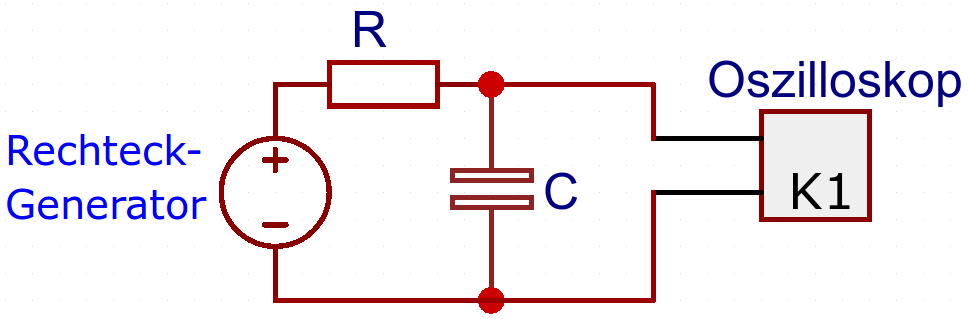
\includegraphics[width=\textwidth]{content/Bilder/Aufbau-1.jpg}
  \caption{Schaltskizze des ersten Versuchsschrittes. Mit \cite{Schaltplanskizzen} erstellt.}
  \label{fig:aufbau1}
\end{figure}
Für die Messung der Zeitkonstanten RC der Schaltung \ref{fig:aufbau1}
wird am Funktionsgenerator eine Rechteckspannung eingestellt.
Die Periodendauer ist so zu wählen, dass sie groß gegen RC ist, auf dem
Oszilloskopbildschirm wird die Zeit $t$ gegen die Spannnung am Kondensator
$U_\text{C}$ aufgetragen. Vom Oszilloskop werden Wertepaare \{$t$, $U_\text{C}(t)$\} von
der Entladekurve genommen.

\newpage

\subsection{Frequenzabhängigkeit von Amplitude und Phase}
\label{sec:messung2}
Das Oszilloskop ist ab jetzt im 2-Kanal Betrieb, wobei $t-x$ und $t-y$ immer
gleichzeitig dargestellt werden.
\begin{figure}
  \centering
  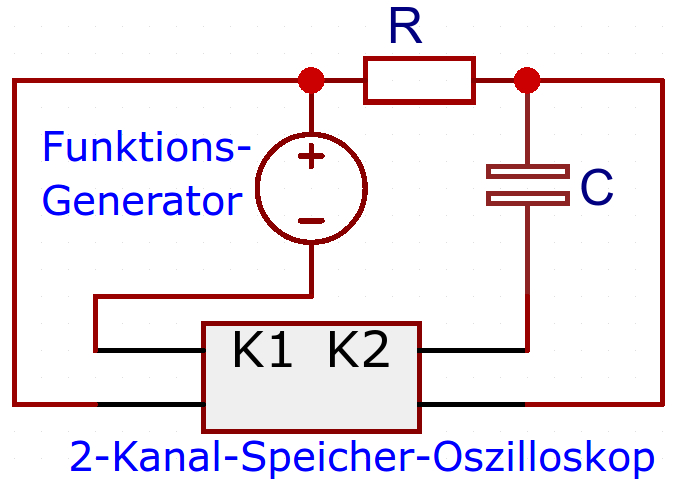
\includegraphics[height=7cm]{content/Bilder/Aufbau-2.jpg}
  \caption{Schaltskizze für alle weiteren Messungen.}
  \label{fig:aufbau2}
\end{figure}\\
Der Funktionsgenerator erzeugt eine Sinusschwingung mit variabler Frequenz.
Gemessen wird jetzt die die Amplitude der Kondensatorspannung $U_\text{C}$ in
Abhängigkeit der Frequenz der anliegenden Sinusspannung, sowie die Phasenverschiebung
zwischen $U \:\text{und}\: U_\text{C}$. Dafür wird der zeitliche Abstand der Extrema
notiert. Zur Überprüfung der Annahme der Konstanz der Amplitude der anliegenden
Spannung wurde diese ebenfalls bestimmt.
Die Messungen erfolgen über 3 Zehnerpotenzen der Frequenz hinweg.


\subsection{Integration}
\label{sec:messung3}
Für die Integration werden Sinus-, Rechteck- und Dreieckspannung benutzt.
Die Frequenz wird auf einen beliebigen Wert, der groß gegen RC ist, gesetzt.

\newpage
